
\chapter{Litt om figurer}\label{kap:figurer}
 
\section{Bruk av \fbox{\tt figure}-miljøet}\label{delkap:figure}
For å inkludere figurer bruker du {\tt figure}-miljøet på følgende
måte

\begin{boxedminipage}{\textwidth}
\begin{verbatim}
\begin{figure}[H]
  \centering
  \scalebox{0.6}{\includegraphics{figurfilnavn}}
  \caption{Figurtekst som beskriver hva vi ser i figuren.} 
  \label{fig:xxxxx}
\end{figure}
\end{verbatim}
\end{boxedminipage}

Den store H-en etter {\tt $\backslash$begin\{figure\}} betyr her,
eller {\em here} på engelsk. Det betyr at figuren plasseres akkurat
der den står i teksten. For å bruke \fbox{[H]} må du inkludere pakken
\fbox{\tt here} på følgende måte \fbox{\tt $\backslash$usepackage\{here\}}.

Dersom du vil at {\LaTeX} skal bestemme plasseringen av figuren ved
kompilering, kan du f.eks. skrive \fbox{[ht]} som betyr at du
\underline{ønsker} at den skal plasseres her og helst mot toppen
øverst på en side. Ved å spesifisere slik havner ofte figuren en helt
annen plass i rapporten, og det er litt slitsomt.

Kommandoen {\tt $\backslash$scalebox\{0.6\}} skalerer figuren til 60\%
av opprinnelig størrelse. 

For oversiktens skyld pleier jeg ofte å la {\tt xxxxx} i figur-{\em tag}'en
\fbox{\tt fig:xxxxx} være det samme som navnet på figurfila, dvs
\fbox{\tt $\backslash$label\{fig:figurfilnavn\}}

\section{MATLAB-figurer}
\subsection{Format og størrelse}
For at MATLAB-figurer skal være lesbar i rapporten må du bruke \fbox{png}-
eller \fbox{pdf}-formatet. Bruker du \fbox{jpg} vil detaljene smøres
utover og  det er ofte umulig å lese ut informasjon av slike
figurer. {\color{red}Inntrykket av rapporten blir dermed dårlig. }
Dersom du lagrer en MATLAB-figur til pdf-formatet ved å bruke
\fbox{\tt File}-menyen som vist i figur~\ref{fig:save_as}, vil det
komme mye tomrom med i figuren som 
vist i  figur~\ref{fig:daarlig}. 

\begin{figure}[H]
  \centering
  \scalebox{0.55}{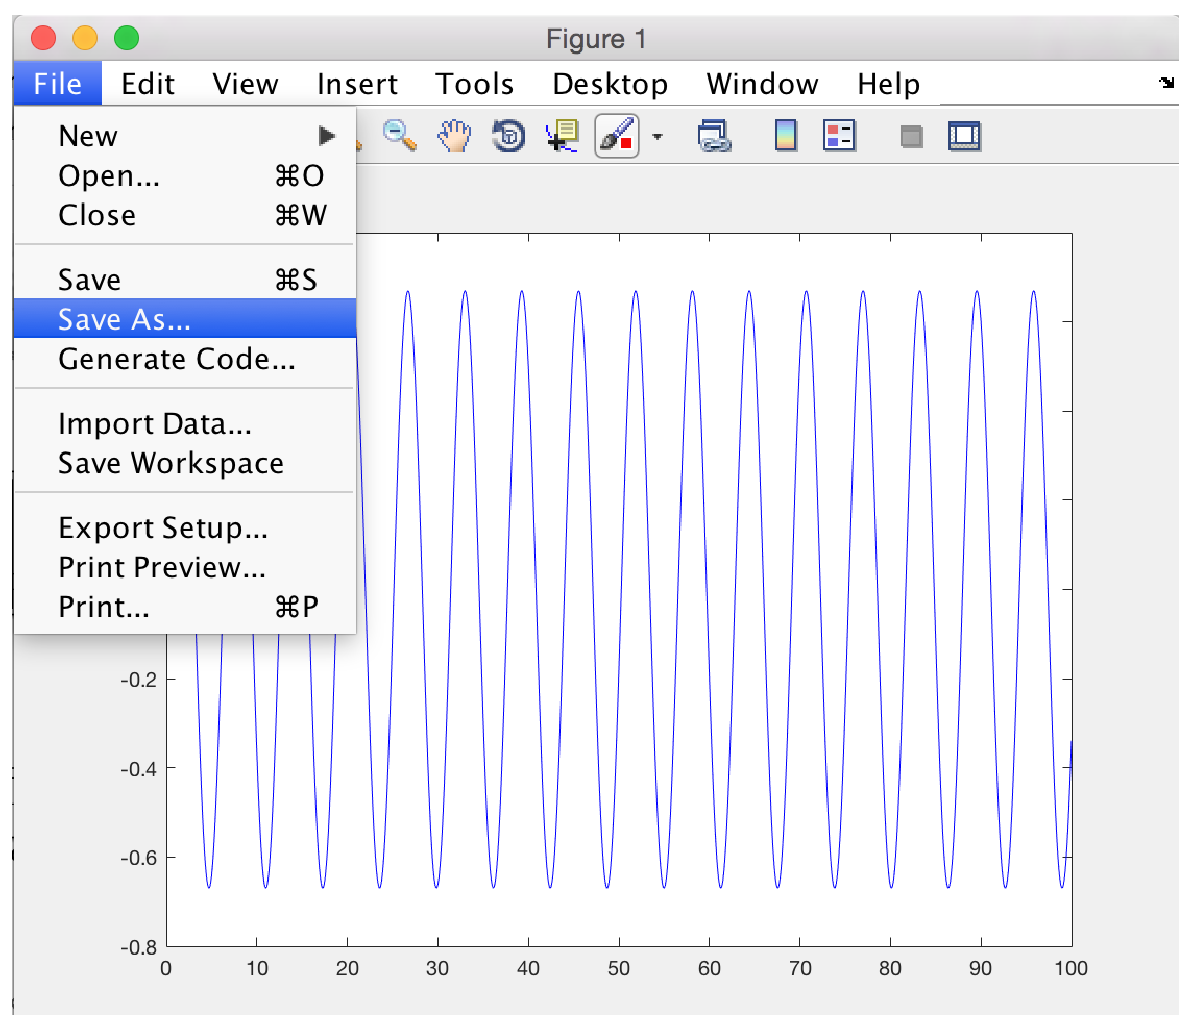
\includegraphics{save_as}}
  \caption{Dersom du lagrer figuren i pdf-format via denne menyen,
    blir det mye hvitt tomrom rundt figuren, se figur~\ref{fig:daarlig}.} 
  \label{fig:save_as}
\end{figure}

\begin{figure}[H]
  \centering
  \scalebox{0.55}{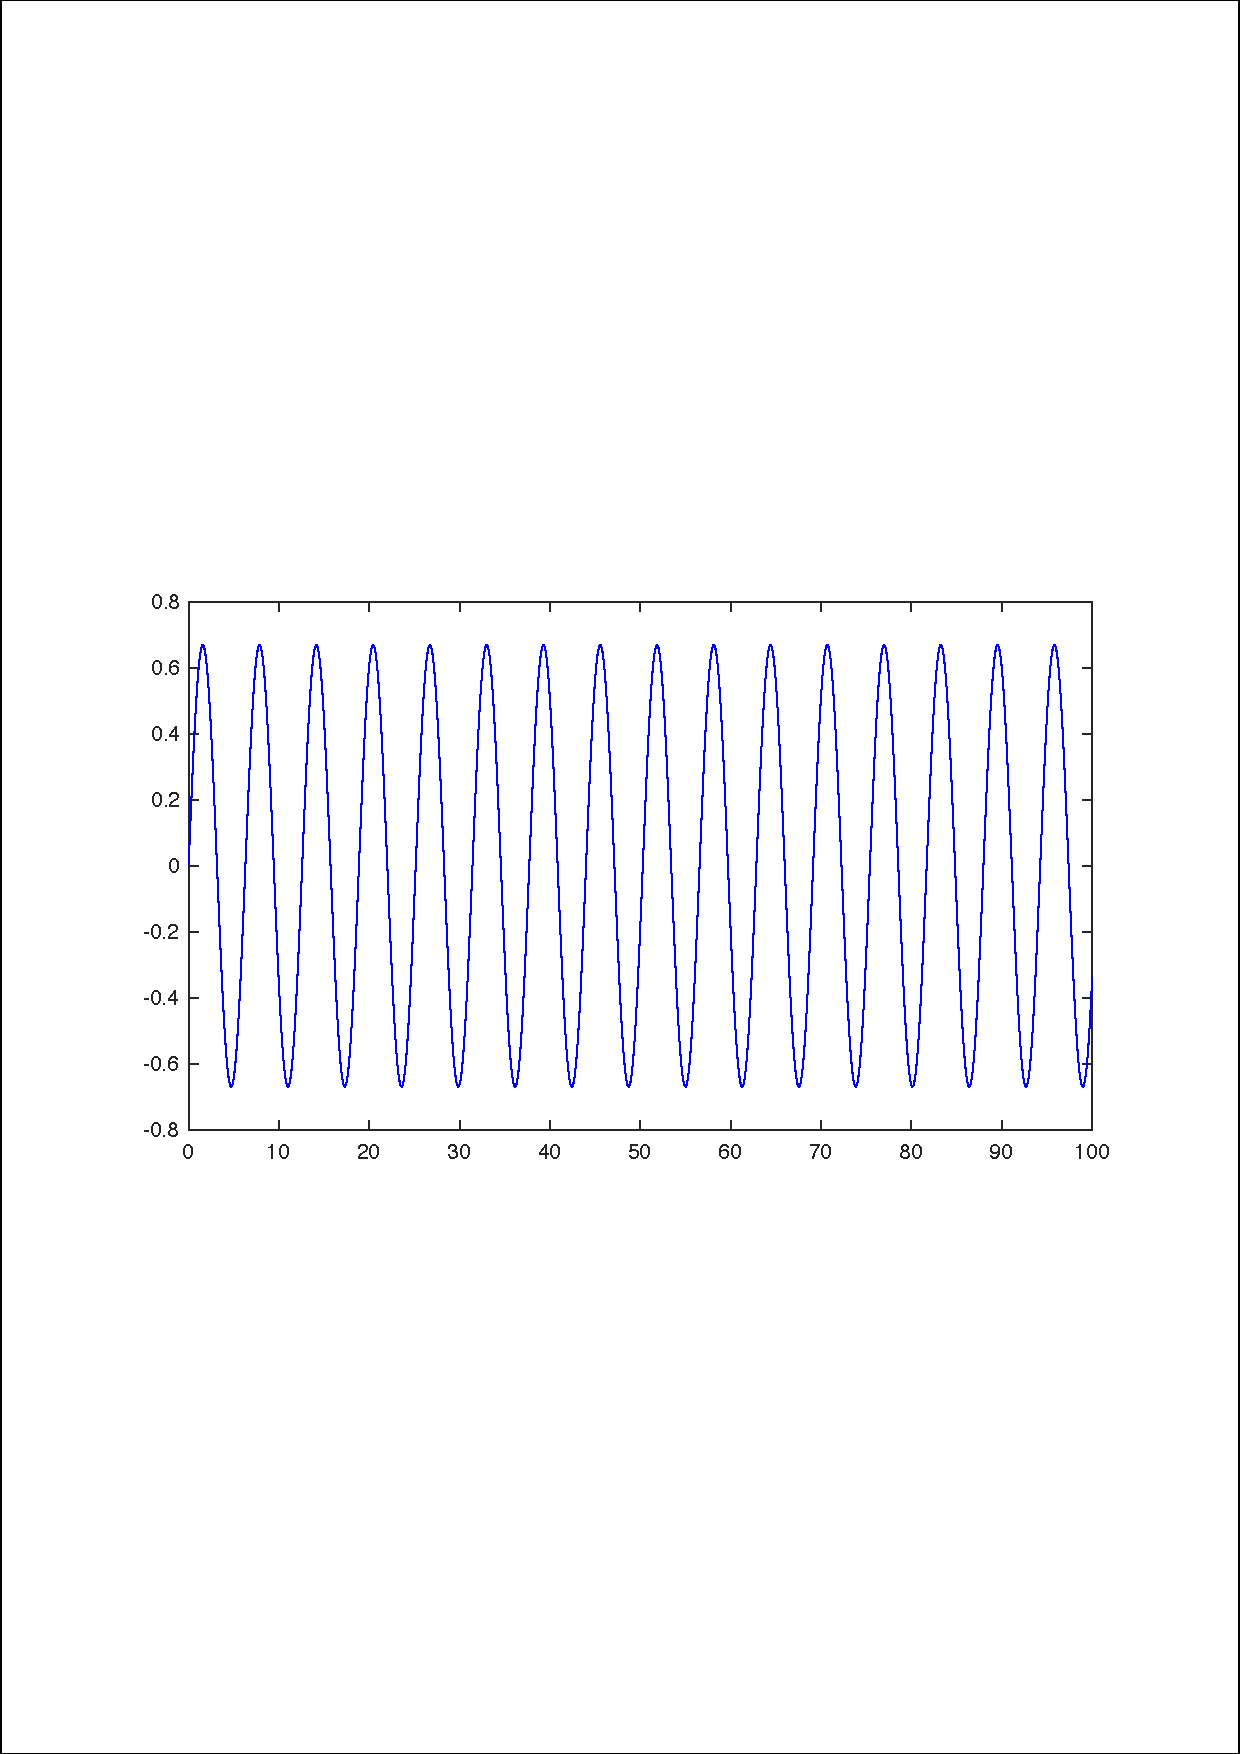
\includegraphics{daarlig_fig}}
  \caption{Dårlig figur med mye hvitt tomrom. Det er lagt
    på en ramme for å vise hvor mye hvitt tomrom som kommer med.} 
  \label{fig:daarlig}
\end{figure}
{\color{red}Dette er med andre ord ikke måten å lage pdf-figurer på.}

\subsection{Funksjonen \fbox{\tt SaveMyFigure.m}}
For at du effektivt skal lage pdf-figurer uten dette store hvite feltet, finner
du i mappen \fbox{MineFunksjoner} en funksjon som heter
\fbox{SaveMyFigure.m}. Denne kaller du med følgende kode i {\em
  Command Window} {\color{red}(husk å stå i den mappen hvor du ønsker
  figuren lagret):}

\begin{boxedminipage}{\textwidth} 
\begin{verbatim}
SaveMyFigure(gcf,'figurnavn')
\end{verbatim}
\end{boxedminipage}

hvor \fbox{\tt gcf} står for \fbox{\tt get current window}, som betyr
at funksjonen lager figur av den MATLAB-figuren du sist trykket med
musepekeren i. Funksjonen lager både en .pdf-versjon
og en .fig-versjon, hvor .fig-versjonen  kan åpnes i ettertid slik at
du ved en 
senere anledning kan endre/legge til ting i figuren.
Koden for funksjonen er i sin helhet gjengitt i
kodeutdrag~\ref{kode:SaveMyFigure}. På side~\pageref{side:kodelisting}
vises det hvordan du kan inkludere kode på denne måten.


\lstinputlisting[caption=Funksjonen {\tt SaveMyFigure.m},
                             label=kode:SaveMyFigure]{SaveMyFigure.m}

\subsection{Effekten av vindusstørrelse {\em før} lagring}
Dersom størrelsen på figuren i forhold til skjermstørrelsen er stor
slik som vist i figur~\ref{fig:god_stort_vindu}, vil resultatet etter lagring med funksjonen
{\tt SaveMyFigure} bli som i figur~\ref{fig:god}
hvor du er at tallene langs x- og y-aksen i figur~\ref{fig:god} nesten
uleselige. 
Dette skyldes at MATLAB-figuren i utgangspunktet dekket nesten hele
skjermen som vist i figur~\ref{fig:god_stort_vindu}.

\begin{figure}[H]
  \centering
  \scalebox{0.22}{\includegraphics{god_stort_vindu}}
  \caption{MATLAB-figuren fyller ut nesten hele skjermen.} 
  \label{fig:god_stort_vindu}
\end{figure}
\begin{figure}[H]
  \centering
  \scalebox{0.21}{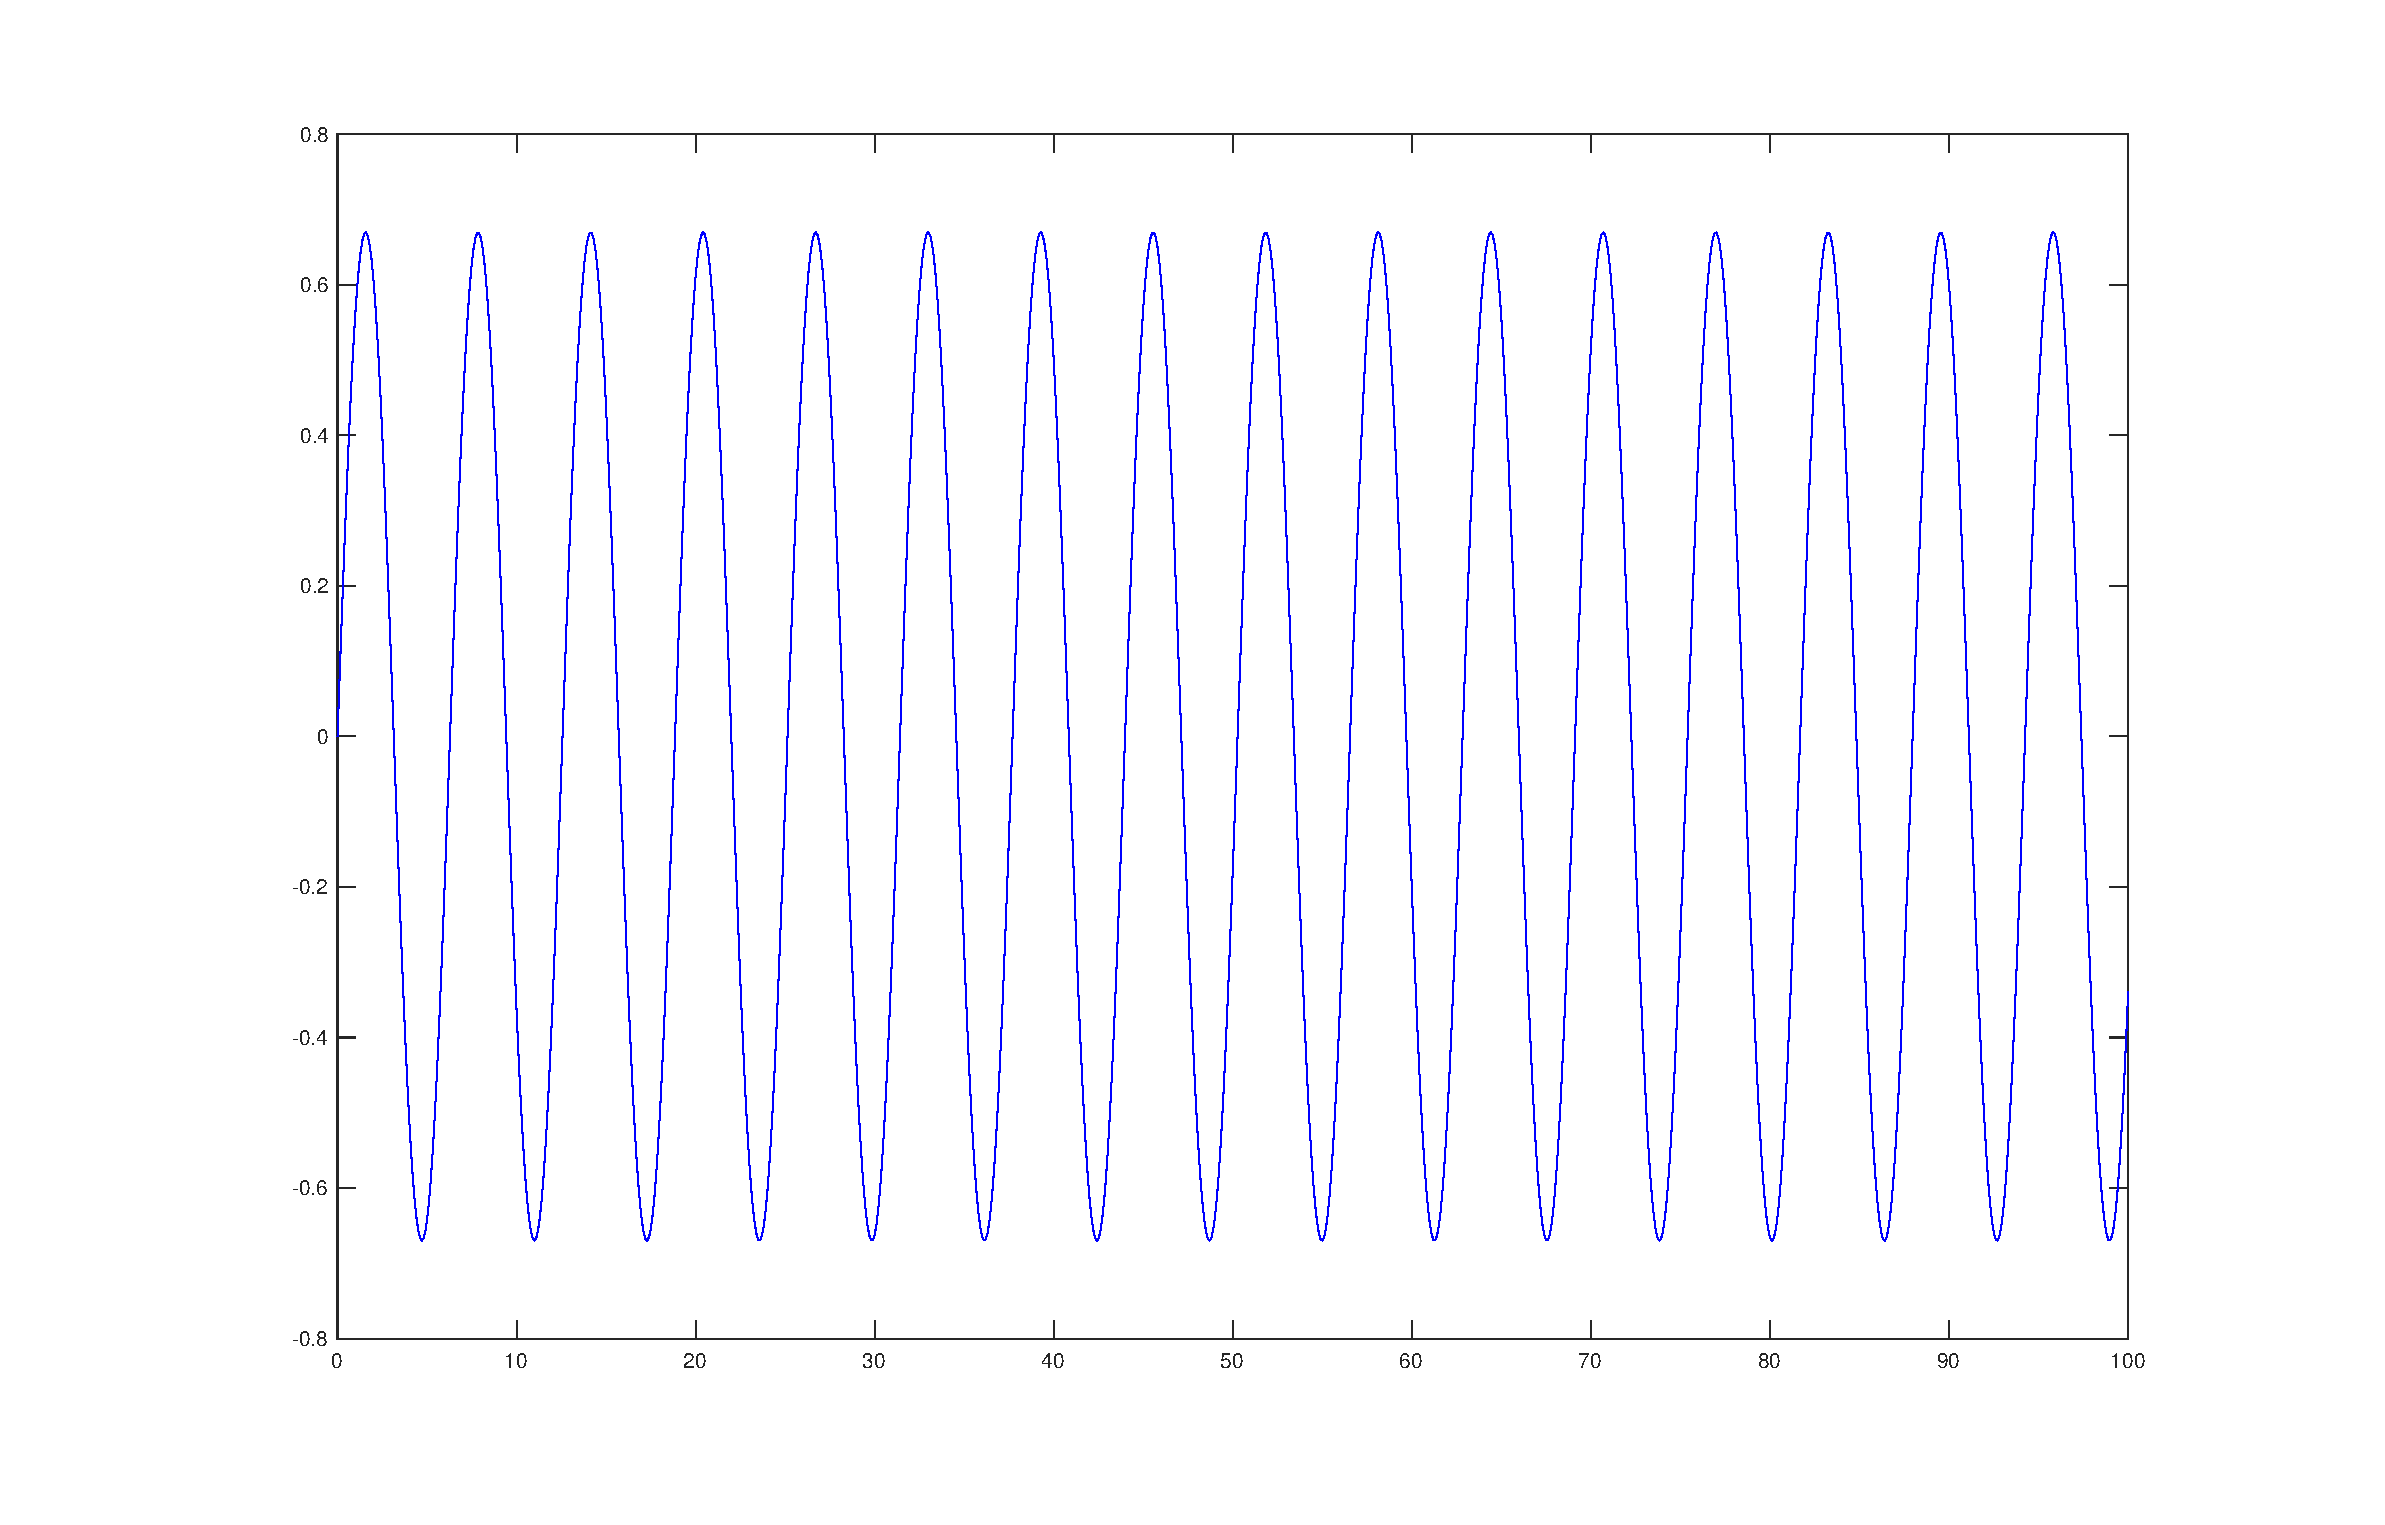
\includegraphics{god}}
  \caption{Slik blir pdf-versjonen av MATLAB-figuren i
    figur~\ref{fig:god_stort_vindu} når lagres med {\tt
      SaveMyFigure}-funksjonen. Tekstfonten er altfor liten, og
    tallverdiene på aksene er uleselig.}  
  \label{fig:god}
\end{figure}

Dersom du reduserer størrelsen på selve MATLAB-figurvinduet 
som vist i figur~\ref{fig:god_lite_vindu} før du lagrer, vil fontstørrelsen på
aksene fremstå som relativt mye større i forhold til selve figuren. 
\begin{figure}[H]
  \centering
  \scalebox{0.22}{\includegraphics{god_lite_vindu2}}
  \caption{MATLAB-figuren er redusert i størrelse før lagring med {\tt
      SaveMyFigure}-funksjonen.} 
  \label{fig:god_lite_vindu}
\end{figure}
Konsekvensen av dette er at leseren
faktisk er i stand til å se tallene, se figur~\ref{fig:god2}.
\begin{figure}[H]
  \centering
  \scalebox{0.58}{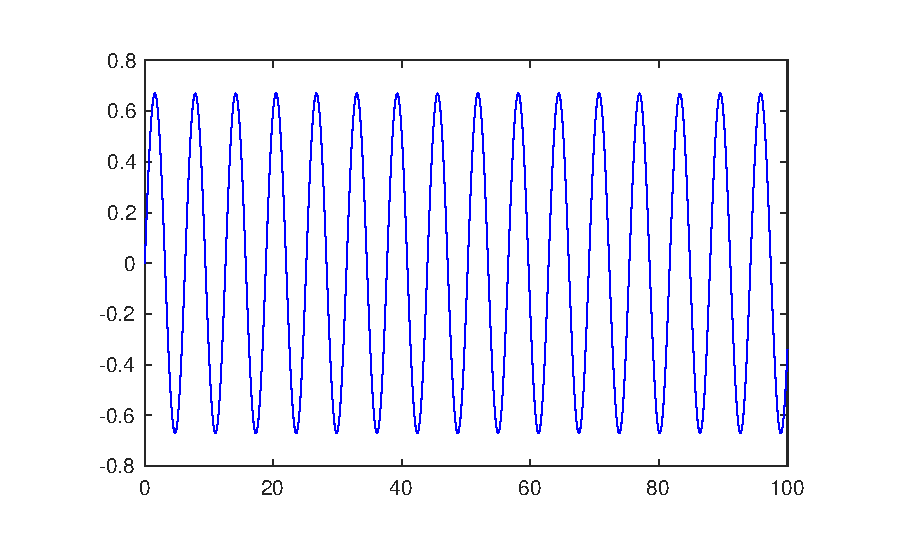
\includegraphics{god2}}
  \caption{MATLAB-figuren i figur~\ref{fig:god_lite_vindu} lagret med {\tt
      SaveMyFigure}-funksjonen. Legg merke til den fornuftige
    fontstørrelsen  på x- og  y-aksen.} 
  \label{fig:god2}
\end{figure}

\subsection{Inkludering av {\LaTeX}-tekst i MATLAB-figurene} 
En figur skal \underline{alltid} ha tekstbasert 
indikering av hva som vises på x- og y-aksene.  I figurene i forrige
delkapittel var dette helt fraværende, og derfor vises det nå
hvordan du kan få {\LaTeX}-font på tekststrengene. Utgangspunktet er
koden for selve sinuskurven i figur~\ref{fig:god2}, men hvor det er
lagt til \fbox{\tt title}, \fbox{\tt xlabel} og \fbox{\tt ylabel} med
{\LaTeX}-font og fontstørrelse 16.

\begin{boxedminipage}{\textwidth}
\begin{verbatim}
t=0:0.1:100;
y_1=2/3*sin(t);
plot(t,y_1)
title('$y_1(t)=\frac{2}{3}\sin(t)$','Interpreter','latex');
xlabel('$t$ [s]','interpreter','latex')
ylabel('$y_1(t)$','interpreter','latex')
\end{verbatim}
\end{boxedminipage}

\begin{figure}[H]
  \centering
  \scalebox{0.58}{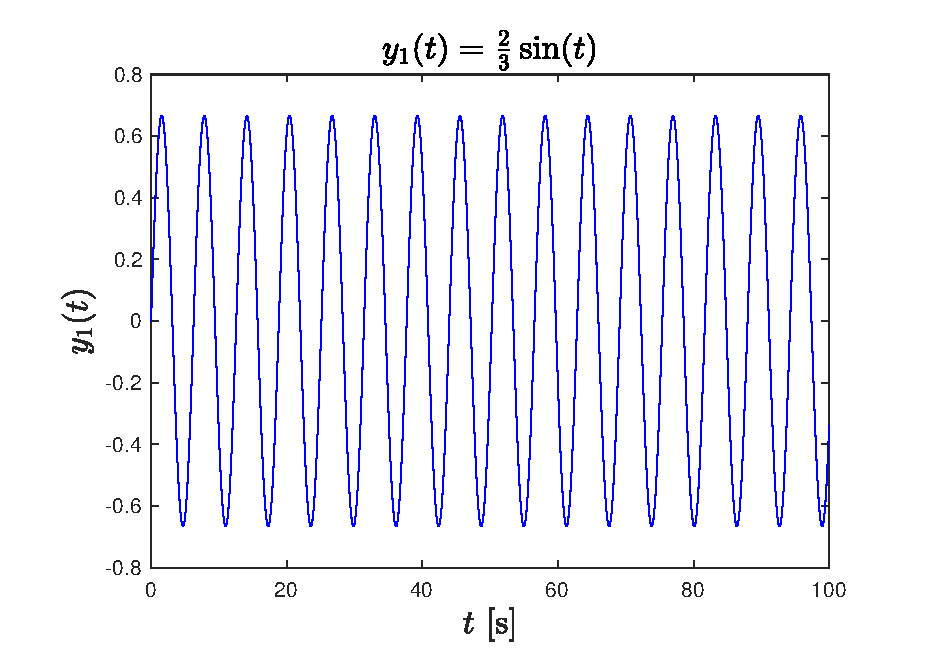
\includegraphics{god3}}
  \caption{Eksempel på en god MATLAB-figur med tydelige, lesbare
    akseverdier og tekst på x- og y-akse, med figurtittel.} 
  \label{fig:god3}
\end{figure}

